\documentclass[a4paper,oneside,11pt]{article}
\usepackage{graphicx}
\usepackage{ tipa }
\usepackage{hyperref}
\usepackage{titling}
\usepackage{blindtext}
\usepackage{enumitem}
\usepackage{eurosym}
\usepackage{float}
\usepackage{listings}
\usepackage{tabularx}
\usepackage{alltt}
\usepackage[T1]{fontenc}
\usepackage{caption}
\usepackage{longtable}
\usepackage{changepage}
\captionsetup[figure]{}


\title{DD}
\author{Daniele Montesi, Nicola Fossati, Francesco Sgherzi}
\date{\today}
\begin{document}
    \begin{titlingpage} 
        \begin{center}
            
\includegraphics[height=5cm]{assets/Logo_Politecnico_Milano.png}\\
            \vspace{4cm}
            \begin{huge} 
                \textbf{\thetitle} \\
            \end{huge}
            \vspace{0.3cm}
                    \begin{Large}
                \textit{Software Engineering 2 Project - TrackMe} \\
            \end{Large}
        \end{center}
         \textbf{v1.0} - 26/12/2018 \\

            \vspace{4cm}
             \begin{large}
            \textbf{Authors}
            \begin{itemize}
                \item Daniele Montesi - \textit{912980} 
                \item Nicola Fossati - \textit{915244}
                \item Francesco Sgherzi - \textit{915377}
            \end{itemize}
        \end{large}
    \end{titlingpage}
    \newpage
    \tableofcontents
    \newpage
    \section{Introduction}
    
        \subsection{Purpose}
            The main purpose of this document is to exhaustively describe the Data4Help main architecture, its parts and how they interact. There is also a chapter that covers the user interface.

The main recipients of this document are the project manager, developers and testers, but it can also be useful for further development reference and maintenance.
        \subsection{Scope}
            % To define the scope of the product we can use ``The World \& Machine'' approach by M. Jackson and P. Zave.
% We can define the real world entities that interact with the system (the World), the entities that belong to the system (the Machine) and the shared phenomena (the intersection of the two other sets).

% TODO: add image here

The \textit{The World and the Machine} approach is used in defining the scope of the project.
By defining the real world entities that interact with the system and the properties of the system itself we can determine the intersection between the two sets: the \textit{shared phenomena}.
\begin{center}
    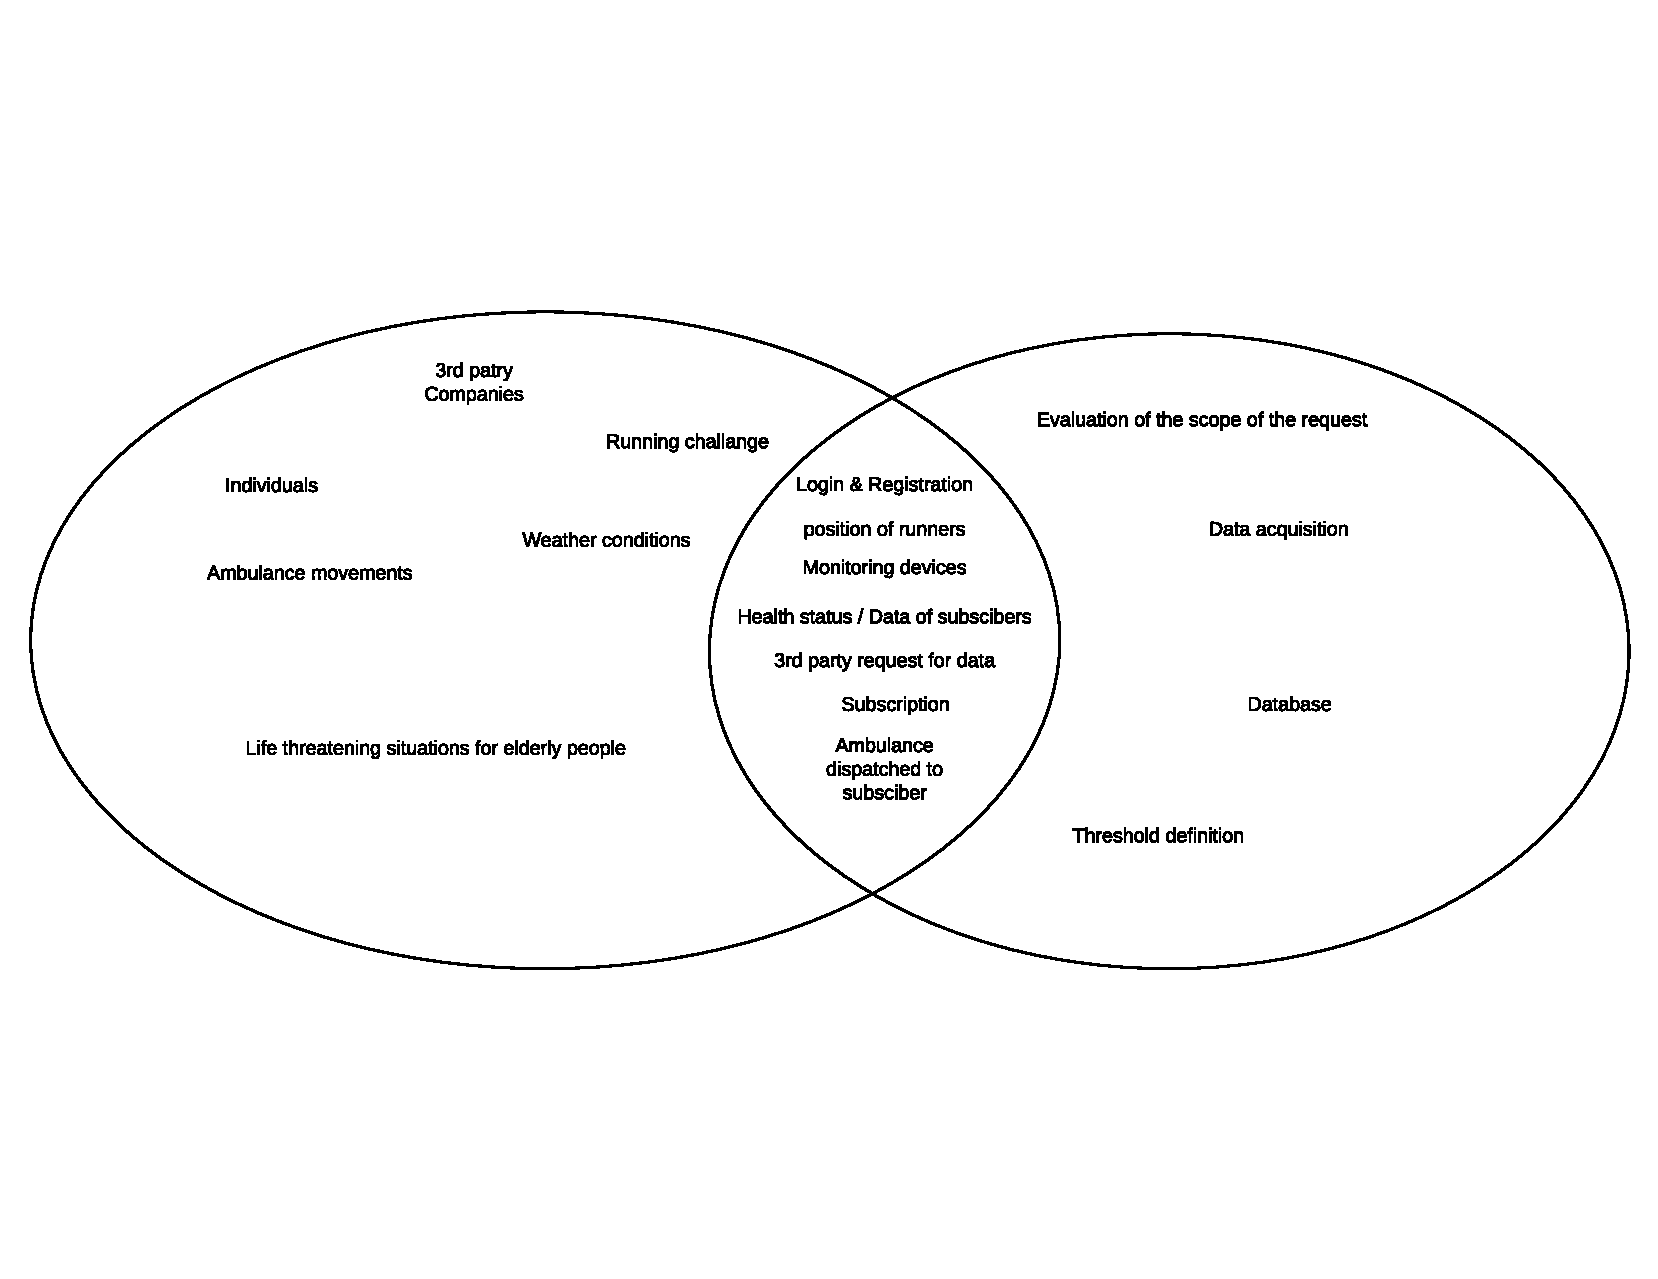
\includegraphics[height=8cm,keepaspectratio]{assets/twatm.pdf}
\end{center}

The system-to-be uses 3 components with different roles in order to work:
\begin{itemize}
    \item \textbf{Data4Help SmartWatch App}: Acquires the data from the smartwatch sensors (heart rate, sleep quality, position, phisical activities) and sends them via Bluetooth to the Data4Help Mobile App
    \item \textbf{Data4Help Mobile App}: Gathers data from the smartwatch, shows various statistics, and sends them to the Data4Help Core Database. Each user can choose which service subscribe to
    \item \textbf{Data4Help Website}: Gives third-party companies the ability to request data, either anonymized or user specific. Moreover, it allows run organizers to define the path of the run and the spectators to see the position of all runners on a map.
    \item \textbf{Data4Help Core}: is intended to connects all other components together providing the logic of the application. It is also responsible for the acceptance of all third-parties requests of data. It also evaluate health status of individuals deciding whether is at risk or not.
\end{itemize}

The list below shows the main goals the system should be able to accomplish:

\begin{itemize}
    \item \textbf{G1}: The system should be able to read sensor data from smart devices.
    \item \textbf{G2}: The system should be able to show acquired data via the Mobile App and the Website.
    \item \textbf{G3}: The system should allow users to register.
    \item \textbf{G4}: The system should allow companies to register.
    \item \textbf{G5}: The system should allow registered companies to request data either from specific individuals or from an anonymized group of individuals.
    \item \textbf{G6}: The system should allow users to accept or decline a company request for their specific data.
    \item \textbf{G7}: The system should provide a payment method to registered companies requesting user data. %eviterei di specificare payment system
    \item \textbf{G8}: The system should be able to communicate directly to ambulances.
    \item \textbf{G9}: The system should be able to react to the lowering of the health parameters below threshold in less than 5 seconds and send the position of the person to the ambulance system. 
    % \item \textbf{G10}: The system should should allow organizers to define the path for the run.
    \item \textbf{G10}: The system should be able to communicate interoperably with its services: \textit{AutomatedSOS} and \textit{Track4Run}
    \item \textbf{G11} The system should allow run organizers to register.
    \item \textbf{G12} If a run organizer is registered, it can define a run i.e. it can define the path that the participants should follow.
    \item \textbf{G13} A user should be able to enroll to a run.
    \item \textbf{G14} Spectators of a run should be able to see each participant's position on a map.
\end{itemize}

%A health data aggregator app that gives the user the ability to monitor all 

%is intended to offer all the functionalities of the service to the individuals, including heart rate monitoring, sleep monitoring




        \subsection{Definitions, Acronyms, Abbreviations}
            \renewcommand{\arraystretch}{1.5}
\begin{center}
    \begin{tabular}{|l|r|}
        \hline
        \textbf{i.e.} & \textit{Id est}, that is  \\
        \hline
        \textbf{w.r.t} & with respect to  \\
        \hline
        \textbf{w.l.o.g.} & without loss of generality \\
        \hline
        \textbf{The company} & TrackMe \\
        \hline
        \textbf{BLE} & Bluetooth Low Energy \\
        \hline
    \end{tabular}
\end{center}
        \subsection{Revision history}
        \subsection{Reference documents}
            \begin{itemize}
\item \textbf{|REFD1|} \href{https://en.wikipedia.org/wiki/Model–view–presenter}{\textbf{MVP}}

\item \textbf{|REFD2|} \href{https://standards.ieee.org/standard/1016-2009.html}{\textbf{IEEE Std 1016-2009 Standard for Information Technology, Systems Design, Software Design Descriptions}}

\item \textbf{|REFD3|} \href{https://it.wikipedia.org/wiki/Representational_State_Transfer}{\textbf{Representational State Transfers}}

\end{itemize}
        \subsection{Document structure}
        This document is divided in the following chapters:
\begin{description}
\item[Implemented requirements] Explains which functional requirements outlined in the RASD are accomplished, and how they are performed.
\item[Design choices] provides reasons about the implementation decisions taken in order to develop the application.
\item[Source code structure] explains and motivates how the source code is structured both in the front end and in the back end.
\item[Testing] provides the main testing cases applied to the the application
\item[REST API] describes the API implemented for the application.
\end{description}
    

\newpage
    \section{Implemented requirements}
    In this section there are described the functionalities implemented w.r.t the requirements listed in the RASD document.
Below there are listed all the functionality of the system, explained in terms of Database, Frontend, Backend handling.



\subsection{Actor Registration}
\begin{itemize}
\item \textbf{Implemented} requirements
        \begin{itemize}
   \item \textbf{[RM$_M$]}: Users can register, after providing a username, a password and a Fiscal Code/Social Security Number and have connected a compatible Smartwatch
    \item \textbf{[R2$_M$]}: Users can only have one account 
    
    %run organizer
  \item \textbf{[R11$_W$]}: Run organizers can register
    
    %company
    \item \textbf{[R1$_W$]}: Companies can register, after providing a username, a password, an email and a company name

%core
    \item \textbf{[R14$_C$]}: Can validates information provided by the user during registration

        \end{itemize}
    \item \textbf{Non-implemented} requirements
    \begin{itemize}
            \item 
        \end{itemize}
\end{itemize}

\paragraph{Database} \mbox{}\\ 
The database stores the actor data in the table "account".
Passwords are hashed and salted in order to avoid a security flaw.
The specific data for each type of actor is stored in specific tables, each for every actor type: individual\_account, company\_account, run\_organizer.
If the registering actor has, for instance, the same email of an actor already present on the database, the transaction is rolled back.
The same can be said for other \texttt{unique} parameters, such as the \texttt{SSN} for the \texttt{individual\_account}

\paragraph{Back-end} \mbox{}\\ 
The server first checks the required parameters for registration, depending on the actor, hashes the password and performs the first insertion into the table reserved for the actor (namely \texttt{individual\_account} \texttt{run\_organizer\_account} \texttt{company\_account}). Then generates a token which is stored and then sent to the actor mail in order to verify the account.
\paragraph{Front-end} \mbox{}\\

\begin{itemize}
    \item \textbf{Application}: 
    \item \textbf{Website}: Company can register through the homepage clicking on a button that opens a modal. After inserting the data, company clicks 'Send' and becomes automatically registered requiring an email verification.
\end{itemize}


\subsection{Actor Authentication}
\begin{itemize}
    \item \textbf{Implemented} requirements
        \begin{itemize}
    \item \textbf{[R1$_M$]}: Users can log-in
    
    %run organizer
    \item \textbf{[R12$_M$]}: Run organizers can login
    
    %company
    \item \textbf{[R2$_W$]}: Companies can log-in

%core

        \end{itemize}
    \item \textbf{Non-implemented} requirements
    \begin{itemize}
            \item 
        \end{itemize}
\end{itemize}

\paragraph{Database} \mbox{}\\ 
The given actor is requested from the database, if the comparison of the stored password and the given one is successful a token is inserted into the \texttt{user\_token} table.

\paragraph{Back-end} \mbox{}\\ 
The server checks the required parameters for the request, then proceedes to compare the hashed and non-hashed provided password. If the compare is successful it creates a token and stores it into the database, otherwise it negates the access to the actor.

\paragraph{Front-end} \mbox{}\\

\begin{itemize}
    \item \textbf{Application}: The application contains, under each subsection, a Login form. The application validates the information, performs the query to the server and show the result of the login. Both Users (individuals) and Run Organizers can log in using the application.
    \item \textbf{Website}: Company can login through the homepage clicking on a button "Sign in" that opens a modal. After inserting the data, company clicks 'Send' and access to the dashboard of his account.
\end{itemize}

\subsection{Individuals Management}

\begin{itemize}
    \item \textbf{Implemented} requirements
        \begin{itemize}
    %individuals
      
    \item \textbf{[R6$_M$]}: Logged-in users can accept/decline a company individual monitoring request
   
   %core
    \item \textbf{[R2$_C$]}: Can send online notifications via email to all users
    

        \end{itemize}
    \item \textbf{Non-implemented} requirements
    \begin{itemize}
    
    
    %core
    \item \textbf{[R1$_C$]}: Can send online notifications via SMS to all users 
    \item \textbf{[R3$_M$]}: Logged-in users can edit their account info
    \item \textbf{[R5$_W$]}: Logged-in companies can update their account information
    \item \textbf{[R3$_C$]}: Can send online notifications via the Mobile app to its users
        \end{itemize}
    %company
    \item \textbf{[R3$_W$]}: Logged-in companies can see their history and account information
        
\end{itemize}

\paragraph{Database} \mbox{}\\
The authorizations for each individual monitoring request is stored in the table individual\_query, in the column "auth", which is boolean (true if accepted, false if rejected, null if not already evaluated).
Back-end accesses column "email" in table account in order to send emails to the users.


\paragraph{Back-end} \mbox{}\\
The \texttt{/queries/query/individual/pending} endpoint allows the user to accept or decline the pending monitoring request.
The server sends online notification to every actor when he registers, in order to verify the email, and to the company that has performed a query when new data are available.

\paragraph{Front-end} \mbox{}\\
\textbf{Application:} Individual users can accept or decline a company monitoring request by the section reachable through the navigation drawer in the Dashboard.\\
\textbf{Website:} Company can see all account information in the panel 'Account' accessible via the navbar through all the pages, after having logged in.\\

\subsection{Company plan subscription }
\begin{itemize}
    \item \textbf{Implemented} requirements
        \begin{itemize}
            \item 
        \end{itemize}
    \item \textbf{Non-implemented} requirements
    \begin{itemize}
    \item \textbf{[R8$_C$]}: Can provide a payment method for data requested by companies.
    \item \textbf{[R15$_C$]}: Can charge companies on their payment method respecting Track4Me pricing policy
        \end{itemize}
\end{itemize}

\paragraph{Database} \mbox{}\\ 
The server answers with the mockup.
\paragraph{Back-end} \mbox{}\\  
\paragraph{Front-end} \mbox{}\\
\textbf{Web site}: The user can see all subscription plan available by clicking in the panel 'Account' accessible via the nav bar through all the pages, after having logged in.
Company can start the purchasing process after clicking "Purchase" under the respective subscription plan.



\subsection{Data management}
\begin{itemize}
    \item \textbf{Implemented} requirements
        \begin{itemize}
    %smartwatch
    
    %core
        \item \textbf{[R4$_C$]}: Can save and store permanently user data
    \item \textbf{[R5$_C$]}: Can receive and store health parameters and geographical position of registered users
     \item \textbf{[R2$_S$]}: App can send data registered locally to Data4Help Mobile App

        \end{itemize}
    \item \textbf{Non-implemented} requirements
    \begin{itemize}
    %smartwatch
    \item \textbf{[R1$_S$]}: App can read data from sensor and store it locally.
     
      \item \textbf{[R5$_M$]}: Logged-in can specify the nature of the daily activities (i.e. running, biking, swimming, hiking)

        \end{itemize}
\end{itemize}

\paragraph{Database} \mbox{}\\  
User data is stored in the tables "accelerometer", "gps\_coordinates", "hear\_rate", "user\_data".


\paragraph{Back-end} \mbox{}\\  
The individual user can send his data via the {indiv/data} endpoint.
The server inserts the user data into the respective table, if well formatted.
Then proceedes to notify the company for new data if the user is in one of the previously posted query.

\paragraph{Front-end} \mbox{}\\
\textbf{Application:} The data is not actually read from the sensors but the app can generate dummy test data and send it to the server, by the Test option in navigator drawer in he Dashboard.\\
\textbf{Web site: }Company can see data relative to their queries or to their monitored individuals right after having performed a query, clicking in the link provided by the server that redirects the user to a XML file containing the data requested.


\subsection{Query management}
\begin{itemize}
    \item \textbf{Implemented} requirements
        \begin{itemize}
    %company
    \item \textbf{[R6$_W$]}: Logged-in companies can query on some group of individuals data
    \item \textbf{[R7$_W$]}: Registered companies can request access to data of individuals
    \item \textbf{[R8$_W$]}: Logged-in companies can access to an individual data, if the user has given approval
    \item \textbf{[R9$_W$]}: Logged-in companies can export data previously queried using Data4Help

    %core
    \item \textbf{[R6$_C$]}: Can execute queries of companies on individuals if the user has accepted the monitoring request from the company
    \item \textbf{[R7$_C$]}: Can execute queries of companies checking if the searches involve more than 1000 anonimyzed users 

        \end{itemize}
    \item \textbf{Non-implemented} requirements
    \begin{itemize}
            \item 
        \end{itemize}
\end{itemize}

\paragraph{Database} \mbox{}\\ 
General information of queries are saved in table "query", while in tables "query\_user", "radius\_query" and "general\_query" are saved the specific information of queries.
The list of users subjected to the query is stored in the \texttt{query\_user} table.

\paragraph{Back-end} \mbox{}\\  
First, the given query is performed to assess feasibility (i.e on a high enough number of user) and then it is inserted in the database.
The list of users subjected to the query is inserted into the database as well.

\paragraph{Front-end} \mbox{}\\
\textbf{Web site}: Company can perform a query for group of individuals in the panel 'Query' accessible via the navbar through all the pages, after having logged in.\\
In the Query page it will appear a button to start a query. When clicked, it opens a modal with all fields to filter query parameters.
If left empty, the filter is just ignored.\\
The user can click "send" in order to perform the query.\\
Same works for single individuals: a company can perform a query clicking in the panel 'Monitoring' accessible via the navbar.

\subsection{Query subscription}
\begin{itemize}
    \item \textbf{Implemented} requirements
        \begin{itemize}
 \item \textbf{[R6bis$_W$]}: Logged-in companies can subscribe to a query data
        \end{itemize}
    \item \textbf{Non-implemented} requirements
    \begin{itemize}
            \item 
        \end{itemize}
\end{itemize}


\paragraph{Database} \mbox{}\\
\paragraph{Back-end} \mbox{}\\


\paragraph{Front-end} \mbox{}\\
\textbf{Web site:} In order to subscribe to a query, a company can simply select the tick-box in the subscription tick-box in the form of the 'Query' panel.
Company can subscribe to a query of group of individuals only, since there is no need to subscribe to single individuals query.

\subsection{Race Management}
\begin{itemize}
    \item \textbf{Implemented} requirements
        \begin{itemize}
        %individuals
    \item \textbf{[R8$_M$]}: Logged-in users can register to a run before the start time
    \item \textbf{[R9$_M$]}: Logged-in users can see a run information
    \item \textbf{[R13$_M$]}: Logged-in run organizers can organize a run
    \item \textbf{[R14$_M$]}: Organizers of a run can define the path and additional information for that run

        \end{itemize}
    \item \textbf{Non-implemented} requirements
    \begin{itemize}
            \item \textbf{[R15$_M$]}: Organizers of a run can start the run
        \end{itemize}
\end{itemize}

\paragraph{Database} \mbox{}\\
Information about a run are stored in the table "run". The checkpoints of the run are saved in the table "run\_check\_point". The subscriptions of each individual to runs are stored in the table "run\_subscription";
\paragraph{Back-end} \mbox{}\\
The \texttt{/runs} endpoint gives the client a way to exploit the requirements specified.
More specifically: 
\begin{itemize}
    \item \textbf{[R8$_W$]}: \texttt{/runs/join} allows the user to join a run, if exists
    \item \textbf{[R9$_W$]}: \texttt{/runs/positions} allows the user to gather informations on the position of the runners in a given run, if exists
    \item \textbf{[R13$_W$]}  \textbf{[R14$_W$]}: \texttt{/runs/} allows a run organizer to create a run, specifying its path, if it is well formed
\end{itemize}
\paragraph{Front-end} \mbox{}\\
\textbf{Application:} The user can register to a nearby run by using the Track4Run functionality reachable from the Dashboard. Here the user can also see the run information. Run Organizers can create a new run from their control panel, clicking the plus icon and defining checkpoints. The run start automatically at the defined time.

\subsection{Users Spectating Race}
\begin{itemize}
    \item \textbf{Implemented} requirements
        \begin{itemize}
        
        %individuals
        
        \item \textbf{[R10$_M$]}: Logged-in users can see participant position on a map, if the run has started


        %core

    \item \textbf{[R13$_C$]}: Can send the position and rank of athletes during a run to spectator's devices.


        \end{itemize}
    \item \textbf{Non-implemented} requirements
    \begin{itemize}
\item \textbf{[R12$_C$]}: Can compute each athlete's rank in a run and send it to each user device.
        \end{itemize}
\end{itemize}

\paragraph{Database} \mbox{}\\
The positions of the users are retrieved exploiting Data4Help functionality, so the data is in the "gps\_coordinates" table.

\paragraph{Back-end} \mbox{}\\
The server requests the runners position from the database for the given run, if exists.

\paragraph{Front-end} \mbox{}\\
\textbf{Application:} The users can see the position of participants on a map by clicking on View on the Track4Run section in the dashboard.

    
\newpage

    \section{Design Choices}
    \input{chapters/3.1.ProgrammingLanguages.tex}
    

\end{document}